\documentclass[journal,12pt,twocolumn]{IEEEtran}
\usepackage{setspace}
\usepackage{gensymb}
\singlespacing
\usepackage[cmex10]{amsmath}
\usepackage{amsthm}
\usepackage{mathrsfs}
\usepackage{txfonts}
\usepackage{stfloats}
\usepackage{bm}
\usepackage{cite}
\usepackage{cases}
\usepackage{subfig}
\usepackage{longtable}
\usepackage{multirow}
\usepackage{enumitem}
\usepackage{mathtools}
\usepackage{steinmetz}
\usepackage{tikz}
\usepackage{circuitikz}
\usepackage{verbatim}
\usepackage{tfrupee}
\usepackage[breaklinks=true]{hyperref}
\usepackage{graphicx}
\usepackage{tkz-euclide}
\usetikzlibrary{calc,math}
\usepackage{listings}
    \usepackage{color}                                            %%
    \usepackage{array}                                            %%
    \usepackage{longtable}                                        %%
    \usepackage{calc}                                             %%
    \usepackage{multirow}                                         %%
    \usepackage{hhline}                                           %%
    \usepackage{ifthen}                                           %%
    \usepackage{lscape}     
\usepackage{multicol}
\usepackage{chngcntr}
\DeclareMathOperator*{\Res}{Res}
\newcommand{\myvec}[1]{\ensuremath{\begin{pmatrix}#1\end{pmatrix}}}
\renewcommand\thesection{\arabic{section}}
\renewcommand\thesubsection{\thesection.\arabic{subsection}}
\renewcommand\thesubsubsection{\thesubsection.\arabic{subsubsection}}
\renewcommand\thesectiondis{\arabic{section}}
\renewcommand\thesubsectiondis{\thesectiondis.\arabic{subsection}}
\renewcommand\thesubsubsectiondis{\thesubsectiondis.\arabic{subsubsection}}
\hyphenation{op-tical net-works semi-conduc-tor}
\def\inputGnumericTable{}                                 %%
\lstset{
%language=C,
frame=single, 
breaklines=true,
columns=fullflexible
}
\begin{document}
\newtheorem{theorem}{Theorem}[section]
\newtheorem{problem}{Problem}
\newtheorem{proposition}{Proposition}[section]
\newtheorem{lemma}{Lemma}[section]
\newtheorem{corollary}[theorem]{Corollary}
\newtheorem{example}{Example}[section]
\newtheorem{definition}[problem]{Definition}
\newcommand{\BEQA}{\begin{eqnarray}}
\newcommand{\EEQA}{\end{eqnarray}}
\newcommand{\define}{\stackrel{\triangle}{=}}
\bibliographystyle{IEEEtran}
\providecommand{\mbf}{\mathbf}
\providecommand{\pr}[1]{\ensuremath{\Pr\left(#1\right)}}
\providecommand{\qfunc}[1]{\ensuremath{Q\left(#1\right)}}
\providecommand{\sbrak}[1]{\ensuremath{{}\left[#1\right]}}
\providecommand{\lsbrak}[1]{\ensuremath{{}\left[#1\right.}}
\providecommand{\rsbrak}[1]{\ensuremath{{}\left.#1\right]}}
\providecommand{\brak}[1]{\ensuremath{\left(#1\right)}}
\providecommand{\lbrak}[1]{\ensuremath{\left(#1\right.}}
\providecommand{\rbrak}[1]{\ensuremath{\left.#1\right)}}
\providecommand{\cbrak}[1]{\ensuremath{\left\{#1\right\}}}
\providecommand{\lcbrak}[1]{\ensuremath{\left\{#1\right.}}
\providecommand{\rcbrak}[1]{\ensuremath{\left.#1\right\}}}
\theoremstyle{remark}
\newtheorem{rem}{Remark}
\newcommand{\sgn}{\mathop{\mathrm{sgn}}}
\providecommand{\abs}[1]{\vert#1\vert}
\providecommand{\res}[1]{\Res\displaylimits_{#1}} 
\providecommand{\norm}[1]{\Vert#1\rVert}
%\providecommand{\norm}[1]{\lVert#1\rVert}
\providecommand{\mtx}[1]{\mathbf{#1}}
\providecommand{\mean}[1]{E[ #1 ]}
\providecommand{\fourier}{\overset{\mathcal{F}}{ \rightleftharpoons}}
%\providecommand{\hilbert}{\overset{\mathcal{H}}{ \rightleftharpoons}}
\providecommand{\system}{\overset{\mathcal{H}}{ \longleftrightarrow}}
	%\newcommand{\solution}[2]{\textbf{Solution:}{#1}}
\newcommand{\solution}{\noindent \textbf{Solution: }}
\newcommand{\cosec}{\,\text{cosec}\,}
\providecommand{\dec}[2]{\ensuremath{\overset{#1}{\underset{#2}{\gtrless}}}}
\newcommand{\myvec}[1]{\ensuremath{\begin{pmatrix}#1\end{pmatrix}}}
\newcommand{\mydet}[1]{\ensuremath{\begin{vmatrix}#1\end{vmatrix}}}
\numberwithin{equation}{subsection}
\makeatletter
\@addtoreset{figure}{problem}
\makeatother
\let\StandardTheFigure\thefigure
\let\vec\mathbf
\renewcommand{\thefigure}{\theproblem}
\def\putbox#1#2#3{\makebox[0in][l]{\makebox[#1][l]{}\raisebox{\baselineskip}[0in][0in]{\raisebox{#2}[0in][0in]{#3}}}}
     \def\rightbox#1{\makebox[0in][r]{#1}}
     \def\centbox#1{\makebox[0in]{#1}}
     \def\topbox#1{\raisebox{-\baselineskip}[0in][0in]{#1}}
     \def\midbox#1{\raisebox{-0.5\baselineskip}[0in][0in]{#1}}
\vspace{3cm}
\title{ASSIGNMENT-2}
\author{Ojaswa Pandey}
\maketitle
\newpage
\bigskip
\renewcommand{\thefigure}{\theenumi}
\renewcommand{\thetable}{\theenumi}
Download all python codes from 
\begin{lstlisting}
https://github.com/behappy0604/Summer-Internship-IITH/tree/main/Assignment-2
\end{lstlisting}
%
and latex-tikz codes from 
%
\begin{lstlisting}
https://github.com/behappy0604/Summer-Internship-IITH/tree/main/Assignment-2
\end{lstlisting}
%
\section{Question No. 2.39}
Construct a quadrilateral MORE where $MO = 6, OR = 4.5, \angle M = 60 \degree, \angle O = 105 \degree$ and $\angle R = 105 \degree$.
%
\section{SOLUTION}

\begin{enumerate}
\item  Let us generalize the given data:
    \begin{align}
    &\angle M= 60\degree=\theta \label{eq1}
    \\
    &\angle O= 105\degree=\alpha
    \\
    &\angle R= 105\degree=\gamma \label{eq2}
    \\
    &\norm{\vec{O}-\vec{M}} =6=a, \label{eq3}
    \\
    &\norm{\vec{R}-\vec{O}} =4.5=b,\label{eq4}
    \\
    &\vec{M}=\myvec{0\\0}, \vec{O}=\myvec{6\\0}
    \end{align}
    \item Also, Let us assume the other two sides as
\begin{align}
 &\norm{\vec{R}-\vec{E}}=c
 \\
  &\norm{\vec{M}-\vec{E}} =d 
  \\
  &\theta= \theta_1 + \theta_2
  \\
  &\delta= 180\degree-\alpha = 75\degree
\end{align}  
    \item Now on calculating, we get
\begin{align}
&\implies \angle E + 270\degree  = 360\degree,
\\
&\implies \angle E = 90\degree\label{eq1}
\end{align}
 \item Now taking sum of all the angles given and \eqref{eq1}  \text{we get}
\begin{align}
\angle M + \angle O +\angle R +\angle E =360\degree
\end{align}
So construction of given quadrilateral is possible as sum of all the angles is equal to $360\degree$.\\
 \item Now, using cosine formula in $\triangle MOR$ we can find RM:
\begin{multline}
\implies {\norm{\vec{R}-\vec{M}}^2}=
\\
{\norm{\vec{M}-\vec{O}}^2}+ \norm{\vec{O}-\vec{R}}^2-2\times\norm{\vec{M}-\vec{O}} \times \norm{\vec{O}-\vec{R}}\cos{O}
\end{multline}
\begin{align}
\implies RM=8.38\\
\implies \theta= \arcsin 31.24\degree
\end{align}
\item Now in $\triangle MER$,we know
 \begin{align}
 \angle M=28.76\degree, \angle E=90\degree.
  \end{align}
  We know that sum of the angles of a triangle is 180\degree
 \begin{align}
     \implies \angle M+ \angle E+ \angle R= 180\degree
 \end{align}
 \begin{align}
     \implies 28.76\degree+90\degree+\angle R= 180\degree
 \end{align}
 \begin{align}
 \implies \angle R=61.24\degree
 \end{align}
 \item Now applying sine law of triangle, we get \\
 EM= 7.34=d \\
\begin{lemma}
Exact co-ordinates of the given \vec{R} and \vec{E} can be expresssed as
\begin{align}
 \vec{R}= \vec{O}+ \abs{b}\times \myvec{\cos\delta\\\sin\delta}
\end{align}
 \begin{align}
 \vec{E}= \vec{M}+ \abs{d}\times \myvec{\cos M\\\sin M}
 \end{align}
 \end{lemma}
 \begin{proof}
 \begin{itemize}
     \item Calculating the co-ordinates of \vec{R}:\\
 \end{itemize}
 The vector equation of a line can be given by as,
 \begin{align}
\implies \vec{R}= \vec{O}+\abs{b}\times \myvec{\cos\delta\\\sin\delta}
 \end{align}
 Putting the values in the above equation we get,
 \begin{align}
     \implies \vec{R}= \myvec{6\\0}+4.5 \times \myvec{0.259\\0.965}
 \end{align}
 \begin{align}
     \implies \vec{R}= \myvec{6\\0}+\myvec{1.16\\4.35}
 \end{align}
 \begin{align}
     \vec{R}= \myvec{7.16\\4.35}
 \end{align}
\begin{itemize}
     \item Calculating the co-ordinates of \vec{E}:\\
 \end{itemize}
 The vector equation of a line can be given by as,
  \begin{align}
     \implies  \vec{E}= \vec{M}+d \times \myvec{\cos M\\\sin M}
 \end{align}
 Putting the values in the above equation we get,
 \begin{align}
     \implies \vec{E}= \myvec{0\\0}+7.34 \times \myvec{0.50\\0.87}
 \end{align}
 \begin{align}
     \implies \vec{E}= \myvec{0\\0}+\myvec{3.67\\6.36}
 \end{align}
 \begin{align}
     \vec{E}= \myvec{3.67\\6.36}
 \end{align}
 \end{proof}
 \item Now, we have the coordinate of vertices M,O,R,E as,
\begin{align}
\vec{M}= \myvec{0 \\ 0}, \vec{O}= \myvec{6 \\ 0},  \vec{R}= \myvec{7.16 \\ 4.35}, \vec{E}= \myvec{3.67 \\ 6.36}.
\end{align}    
    \item On constructing the given quadilateral on python and marking angle we get:
\end{enumerate}
\numberwithin{figure}{section}
\begin{figure}[!ht]
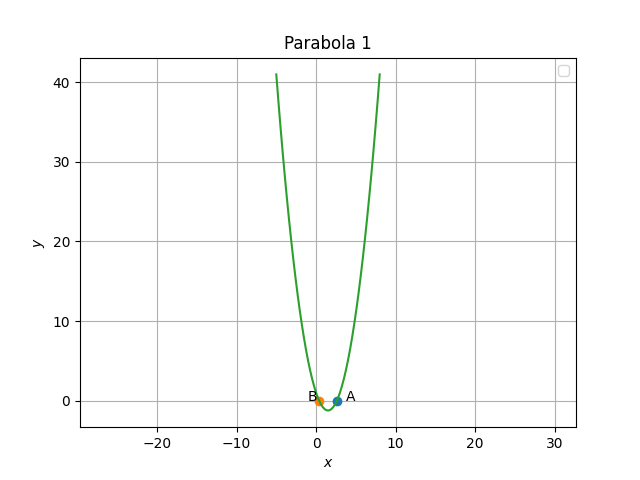
\includegraphics[ width=\columnwidth, height=6 cm]{figure.png}
\caption{Quadrilateral MORE}
\label{fig:Quadrilateral MORE}	
\end{figure}
\end{document}
